%********************************************************************
% Appendix
%*******************************************************
% If problems with the headers: get headings in appendix etc. right
%\markboth{\spacedlowsmallcaps{Appendix}}{\spacedlowsmallcaps{Appendix}}
\chapter[Expérience annexe: congruence]{Influence de la congruence sur la détection des événements sonores}
\label{app:xp_congruence}


\section{Objectif de l'expérience}

Une étude réalisée par \citep{gygi2011incongruency}, tend à montrer que les sons incongrus dans un environnement sonore ambiant (canard dans aéroport) sont plus facilement reconnaissables que des sons naturellement adaptés (avion dans aéroport). Ils nomment cet effet, l'avantage de l'incongru (AI). Pour démontrer cela, ils ont effectué un certain nombre d’expériences sur une population élargie, en demandant aux individus d’identifier la nature d’un son court dans une scène longue, parmi un liste de réponses forcées. La seule condition expérimentale variant est le rapport noté $\dfrac{So}{Sb}$ entre le niveau du son cible à identifier ($So$), et celui du fond sonore ($Sb$).

L'objectif de cette expérience est d'introduire une nouvelle variable à l'étude réalisée par \citep{gygi2011incongruency}, à savoir la position du son cible à reconnaître dans la scène. Il est en effet possible que l'AI dépende du temps d'exposition du sujet à l'environnement ambiant. 

Nous faisons l'hypothèse que, plus le temps d'exposition précédant le son cible est long, plus l'AI sera élevé. Cet effet pouvant dépendre de la durée totale de la scène, nous considérons 3 conditions expérimentales:

\begin{itemize}
\item la durée de la scène: nous considérons deux valeurs de $5$ et $10$ secondes;
\item la position du son cible: nous considérons trois valeurs correspondant au début, au milieu et à la fin de la scène. Le calcul des positions dépend de la durée de la scène :

\begin{itemize}
\item pour une durée de 5 secondes: début$=0.5$ seconde, milieu$=2.25$ secondes, fin$=3.5$ secondes;
\item pour une durée de 10 secondes: début$=1$ seconde, milieu$=4$ secondes, fin$=7$ secondes;
\end{itemize}

\item la congruence: nous considérons deux valeurs, congru et incongru, suivant que le son cible est adapté ou non à l'environnement ambiant.
\end{itemize}

\section{Banque de données}

Nous considérons une banque de données composée de 8 enregistrements d'ambiances et de 8 enregistrements de sons isolés, ces derniers correspondant aux sons cibles à identifier. La moitié de ces enregistrements est prévue pour des scènes longues (ambiance: 10 secondes, sons cibles: 2 secondes), l'autre moitié pour des scènes courtes (ambiance: 5 secondes, sons cibles: 0.5 secondes).

Cibles et ambiances ont été choisies de sorte que toutes les cibles puissent être introduites et dans une scène congrue, et dans une scène incongrue. Pour chaque association cible/ambiance, trois scènes sont simulées réservant chacune une position différente au son cible (début, milieu et fin). Enfin chaque scène est simulée deux fois en considérant des ratios $\dfrac{So}{Sb}$ de $-6$ et $-9dB$.

Cette procédure de simulation nous donne une banque de sons de 96 scènes simulées (8*2*3*2). A noter cependant qu'un même sujet n'est soumis qu'à des scènes partageant le même $\dfrac{So}{Sb}$, soit 48 scènes.


\section{Planification expérimentale}

{\setlength{\parindent}{0cm}\textbf{Procédure}} \\ 

Pour chacune des 48 scènes, le sujet doit identifier le son cible parmi 15 réponses proposées. Ce choix des 15 réponses, quand il n'y a que 8 cibles, a été fait de manière 1) à limiter les effets de mémoire, 2) à empêcher que le sujet procède par élimination.

Afin que le sujet puisse identifier les cibles, il est nécessaire de lui indiquer quand celles-ci surviennent dans la scène. Une interface graphique a été développée à cet effet. Elle permet d'afficher les 15 réponses possibles, ainsi qu'un voyant qui s'allume au vert lorsque le son cible est joué. Cette méthode est jugée moins invasive que celle proposée par \citep{gygi2011incongruency}, où l’apparition du son cible dans la scène est précédée d'un court son pur.

Les scènes sont présentées dans un ordre aléatoire. \\

{\setlength{\parindent}{0cm}\textbf{Dispositif expérimental}} \\

Tous les sujets passent l'expérience sur des machines identiques. L'audio est diffusé en monophonique, par le biais de casques audio semi-ouverts \emph{Beyer-Dynamic DT 990 Pro}. 

Les sujets passent l'expérience individuellement, dans un environnement acoustique calme. Un expérimentateur est présent durant la totalité de l'expérience, afin de contrôler son bon déroulement, et de répondre aux éventuelles questions des sujets. \\

{\setlength{\parindent}{0cm}\textbf{Participants}} \\

15 sujets ont passé l'expérience pour un $\dfrac{So}{Sb}=-6dB$, et 15 autres pour un $\dfrac{So}{Sb}=-9dB$. Tous les sujets sont des étudiants de l'École centrale de Nantes.

\section{Méthodologie et outils statistiques}

Pour chaque condition expérimentale, et chaque sujet, nous calculons le pourcentage de réponses correctes noté $p(c)$.

Pour apprécier s'il existe des différences entre les conditions expérimentales au niveau des moyennes de $p(c)$ relevées, nous considérons une ANOVA à mesures répétées à trois facteurs, nommément, la durée, la position et la congruence. La sphéricité est évaluée à l'aide du test de Mauchly. Si cette dernière n'est pas vérifiée, la correction de Greenhouse-Geisser est appliquée, la valeur $p$ est alors notée $p_{gg}$. Le seuil de significativité est fixé à $\alpha=0.05$.

\section{Résultats}

\begin{figure}[t]
        \myfloatalign
        \subfloat[]
        {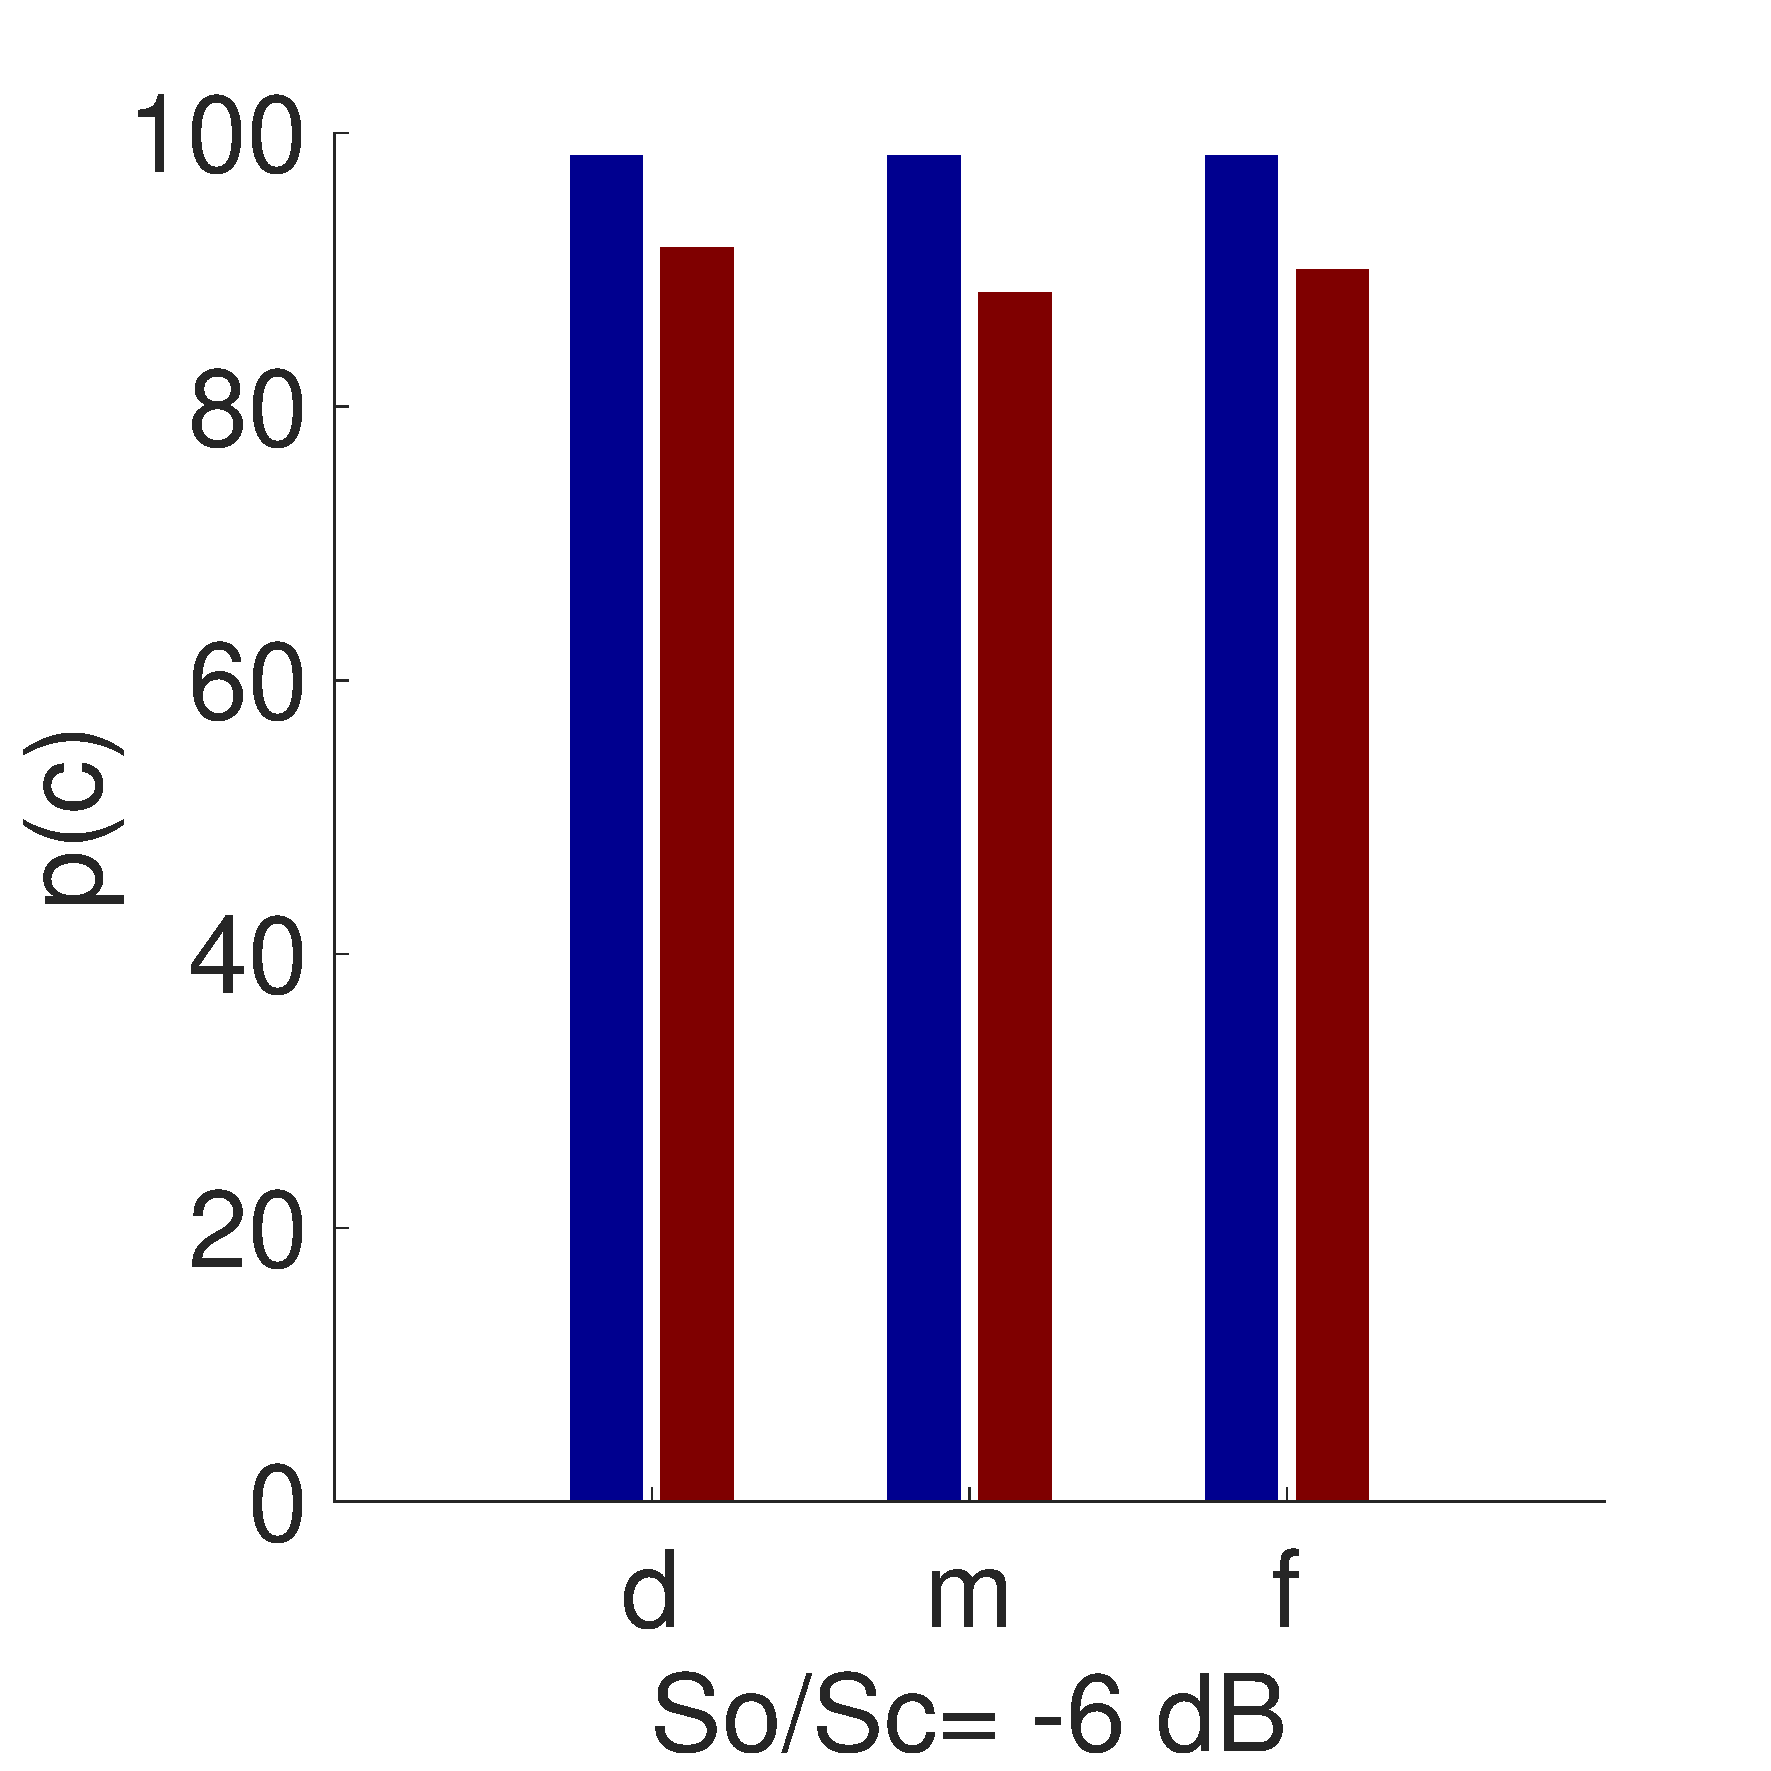
\includegraphics[width=.5\linewidth]{gfx/app_congruence/xpCongruence_3}\label{fig:xpCongruencea}}
        \subfloat[]
        {\includegraphics[width=.5\linewidth]{gfx/app_congruence/xpCongruence_4}\label{fig:xpCongruenceb}} \par
        \subfloat[]
        {\includegraphics[width=.5\linewidth]{gfx/app_congruence/xpCongruence_1}\label{fig:xpCongruencec}}
        \subfloat[]
        {\includegraphics[width=.5\linewidth]{gfx/app_congruence/xpCongruence_2}\label{fig:xpCongruenced}} \par
        \caption[Pourcentage de réponses correctes en fonction de la position du son cible et de la congruence.]{Pourcentage de réponses correctes en fonction de la position du son cible et de la congruence; En considérant $\dfrac{So}{Sb}=-6dB$ (a, b), $\dfrac{So}{Sb}=-9dB$ (c, d), des scènes longues (b, d) et des scènes courtes (a, c).}\label{fig:xpCongruence}
\end{figure}

Concernant $\dfrac{So}{Sb}=-6dB$, l'ANOVA à mesures répétées montre un effet significatif de la congruence ($F[1,14]=9$ ,$p<0.05$), de la durée des scènes ($F[1,14]=21$ ,$p<0.01$), mais pas de la position du son cible ($F[2,28]=2$ ,$p_{gg}=0.17$) (\cf~Figures~\ref{fig:xpCongruencea} et~\ref{fig:xpCongruenceb}).

Les mêmes résultats sont observés pour $\dfrac{So}{Sb}=-9dB$, avec un effet significatif de la congruence ($F[1,14]=15$ ,$p<0.01$), de la durée des scènes ($F[1,14]=64$ ,$p<0.01$), mais pas de la position du son cible ($F[2,28]=2$ ,$p_{gg}=0.15$) (\cf~Figures~\ref{fig:xpCongruencec} et~\ref{fig:xpCongruenced}).

Plusieurs points sont à retenir. Premièrement, nous retrouvons bien l'AI de \citep{gygi2011incongruency}, et ce pour presque toutes les conditions expérimentales. Deuxièmement, nous observons un effet du rapport $\dfrac{So}{Sb}$ cohérent, \ie~plus le niveau du son cible est fort, par rapport à celui de la scène, et plus le $p(c)$ augmente. Troisièmement, plus la durée de la scènes est courte, et plus $p(c)$ augmente.

Nous ne relevons pas d'effet significatif de la position. Cependant la figure~\ref{fig:xpCongruence} nous permet d'apprécier qualitativement certaines tendances. On peut voir que l'effet de la position varie suivant que l'on considère une scène courte (\cf~Figures~\ref{fig:xpCongruencea} et~\ref{fig:xpCongruencec}), ou une scène longue (\cf~Figures~\ref{fig:xpCongruenceb} et~\ref{fig:xpCongruenced}). Dans le cas d'une scène courte, aucune tendance ne semble se dégager. En revanche, dans le cas d'une longue, plus la position est éloignée dans le temps, et plus l'AI se réduit. Ces dernières observations nous permettent de conjecturer deux points. Si l'AI dépend de la position du son cible, alors:

\begin{itemize}
\item il dépend également de la durée de la scène. Pour une durée courte (5 secondes), la position est négligeable;
\item plus la position est éloignée dans le temps et plus l'AI se réduit. On constate ainsi l'inverse de notre hypothèse de départ. Il semblerait que plus le sujet a le temps de se familiariser avec l'environnement, et moins le caractère incongru d'un son favorise son identification. 
\end{itemize}